
	\section{Понятие о когерентности. Частично когерентный свет. Основные интерференционные
		схемы. Интерференция плоских волн, пространственный период полос.}
	Монохроматических волн не бывает в природе. В реальности волны часто излучаются модулированными как по амплитуде, так и по частоте. Такие называют квазимонохроматическими. 
	\begin{align*}
	a(t) \cos (\omega t + b(t))
	\end{align*}
	\textbf{когерентными наз ывают две волны, если у них постоянная разность фаз}\\
	Так две монохроматические волны когерентны, если у них одинаковая частота.\\
	Если есть какая-то маленькая разница в частотах $\Delta \omega$ то говорят о времени когерентности $t \Delta \omega \sim \pi$. Предполагаю малость $\Delta \omega$ получаем $t \sim \dfrac{\lambda^2}{2c \Delta \lambda}$ отсюда получается то, что называют длинной когерентности $l \sim \dfrac{\lambda^2}{2\Delta \lambda}$\\
	Пусть у нас есть две плоские волны. 
	\begin{align*}
	A_1 = a_1 \cos \mathbf{k_1 r} - \omega t + \phi_1\\
		A_2 = a_2 \cos \mathbf{k_2 r} - \omega t + \phi_2
	\end{align*}
	Тогда не сложно их сложить и получить распределение интенсивности
	\begin{align*}
	I = I_1 + I_2 + 2\sqrt{I_1 I_2} \cos( \mathbf{(k_1 - k_2)r} + \phi_1 - \phi_2 )
	\end{align*}
	Ага, теперь мы знаем, что интенсивность постоянна в плоскостях перпендикулярных $\mathbf{k_1 - k_2}$ \\
	Расстояние между плоскостями максимумов будет $\dfrac{2\pi}{|\mathbf{k_1 - k_2}|}$. Для равных по модулю векторов $\dfrac{\lambda}{2 \sin \alpha/2}$ где альфа это угол между векторами\\
	\subsection{Основные схемы}
	\textbf{Схема Юнга.} 
	\begin{figure}[h]
		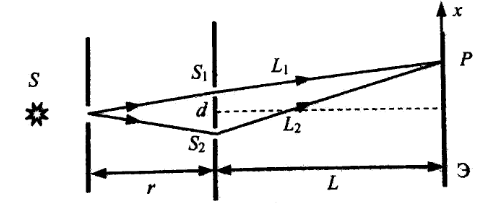
\includegraphics[scale = 0.7]{17_1}
	\end{figure}
	Ширина полос и расстояние между ними равно $\dfrac{\lambda L}{d}$\\ 
	\textbf{Тонкий клин.} В приближении малых углов падения и малости угла альфа просто поворачивает входной луч на $(n-1)\alpha$\newpage
	\begin{figure}[h]
		\centering
		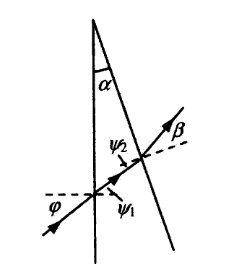
\includegraphics[scale = 0.7]{17_2}
	\end{figure}
	\textbf{Бипризма Френеля} Две призмы из прошлого пункта. В итоге получаем, что эффективно один источник расслаивается на два. Расстояние между ними $2a(n-1)\alpha$, и теперь задача свелась просто к опыту Юнга \\
	\begin{figure}[H]
		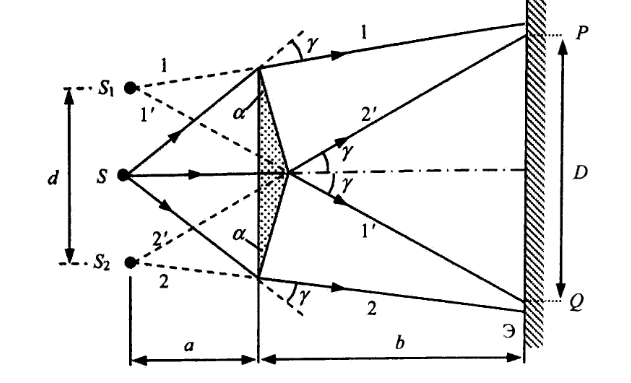
\includegraphics[scale = 0.5]{17_3}
	\end{figure}
